\documentclass[aspectratio=169]{beamer}

%==================================
% THEME AND COLOR
%==================================
\usetheme{Boadilla}
\usecolortheme{beaver}
\setbeamertemplate{blocks}[rounded][shadow=true]

%==================================
% PACKAGES
%==================================
\usepackage{graphicx}
\usepackage{listings}
\usepackage{xcolor}
\usepackage{booktabs}
\usepackage{tikz}
\usetikzlibrary{arrows.meta, positioning, calc}
\usepackage{fontawesome5}

%==================================
% CUSTOMIZATION
%==================================
\definecolor{codegreen}{rgb}{0,0.6,0}
\definecolor{codegray}{rgb}{0.5,0.5,0.5}
\definecolor{codepurple}{rgb}{0.58,0,0.82}
\definecolor{backcolour}{rgb}{0.98,0.98,0.97}

\lstdefinestyle{mystyle}{
    backgroundcolor=\color{backcolour},
    commentstyle=\color{codegreen},
    keywordstyle=\color{magenta},
    numberstyle=\tiny\color{codegray},
    stringstyle=\color{codepurple},
    basicstyle=\ttfamily\footnotesize,
    breaklines=true,
    keepspaces=true,
    numbers=left,
    numbersep=5pt,
    showspaces=false,
    showstringspaces=false,
    showtabs=false,
    tabsize=2
}
\lstset{style=mystyle}

%==================================
% TITLE INFORMATION
%==================================
\title[Git \& GitHub]{\textbf{Mastering Git \& GitHub: From Zero to Collaboration}}
\subtitle{A Comprehensive Hands-on Course}
\author{Abderrahman Bouanani \&\& Houcine Gahboub}
\institute{ENSAA}
\date{\today}

%==================================
% DOCUMENT START
%==================================
\begin{document}

\begin{frame}
  \titlepage
\end{frame}

\begin{frame}{Course Overview}
  \begin{itemize}
    \item Understand version control concepts
    \item Master Git commands and workflows
    \item Collaborate effectively using GitHub
    \item Handle real-world scenarios
    \item Learn best practices and troubleshooting
  \end{itemize}
\end{frame}

\begin{frame}{Course Structure}
  \tableofcontents
\end{frame}

%=======================
\section{Session 1: Version Control \& Git Fundamentals}
%=======================

\begin{frame}{Learning Objectives}
  \begin{columns}
    \begin{column}{0.6\textwidth}
      \begin{block}{By the end of this session, you will be able to:}
        \begin{itemize}
          \item Explain the importance of version control
          \item Set up and configure Git
          \item Create and manage repositories
          \item Track changes with commits
        \end{itemize}
      \end{block}
    \end{column}
    \begin{column}{0.35\textwidth}
      
\includegraphics[width=\textwidth]{figures/gitGithub.png}
    \end{column}
  \end{columns}
\end{frame}

\begin{frame}{Why Version Control?}
\begin{block}{Scenario: The "One Small Change" Problem}
\begin{itemize}
  \item Your program is working perfectly.
  \item You change "just one little thing"...
  \item Your program breaks.
  \item You try to change it back...
  \item \alert{Your program is still broken!}
\end{itemize}
\end{block}
\end{frame}

\begin{frame}{What is Version Control?}
  \begin{block}{A system that records changes to files over time}
    Think of it as a \textbf{time machine} for your code!
  \end{block}
  
  \begin{columns}
    \begin{column}{0.5\textwidth}
      \begin{block}{Key Features}
        \begin{itemize}
          \item \textbf{History}: See who changed what and when.
          \item \textbf{Backup}: Recover any previous version.
          \item \textbf{Collaboration}: Work with others seamlessly.
        \end{itemize}
      \end{block}
    \end{column}
    \begin{column}{0.45\textwidth}
      \begin{exampleblock}{Analogy}
        Like "Track Changes" in a document, but supercharged for code.
      \end{exampleblock}
    \end{column}
  \end{columns}
\end{frame}




% Git Introduction
\begin{frame}{What is Git?}
  \begin{block}{A distributed version control system}
    \begin{itemize}
      \item Created by Linus Torvalds in 2005
      \item Initially developed for Linux kernel development
      \item Now the most widely used VCS in the world
    \end{itemize}
  \end{block}
  
  \vspace{1em}
  \begin{center} 
    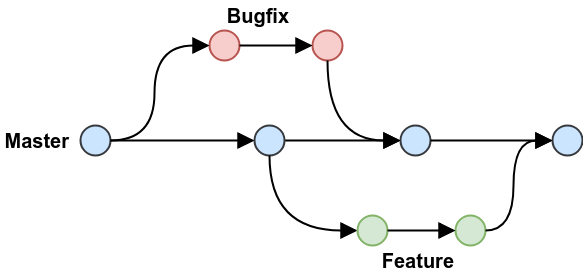
\includegraphics[width=0.5\textwidth]{figures/gitWorkflowDiagram.png}
  \end{center}
\end{frame}


%--- Core Git Concepts ---
\begin{frame}{Core Git Concepts: The Three Areas}
  \centering
  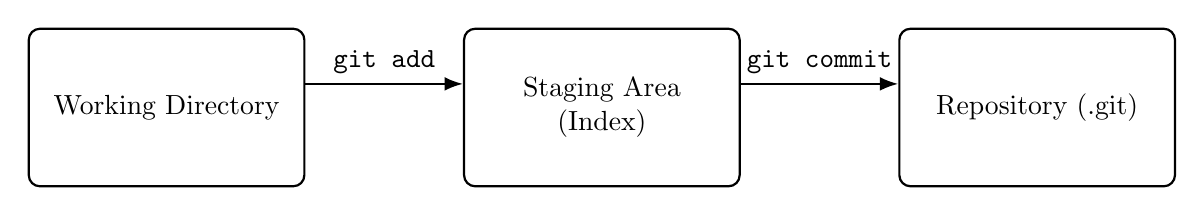
\begin{tikzpicture}[
    node distance=2cm,
    area/.style={rectangle, draw, thick, rounded corners, minimum height=2cm, minimum width=3.5cm, text width=3cm, align=center},
    arrow/.style={-Latex, thick}
  ]
    \node[area] (wd) {Working Directory};
    \node[area, right=of wd] (sa) {Staging Area (Index)};
    \node[area, right=of sa] (repo) {Repository (.git)};

    \draw[arrow] ($(wd.east)+(0,0.3)$) -- node[above] {\texttt{git add}} ($(sa.west)+(0,0.3)$);
    \draw[arrow] ($(sa.east)+(0,0.3)$) -- node[above] {\texttt{git commit}} ($(repo.west)+(0,0.3)$);
  \end{tikzpicture}
  \begin{itemize}
      \item \textbf{Working Directory}: Files you actively modify.
      \item \textbf{Staging Area}: Draft of your next commit.
      \item \textbf{Repository}: Full history stored in .git.
  \end{itemize}
\end{frame}

%--- Essential Git Commands ---
\begin{frame}{Essential Git Commands}
  \begin{columns}
    \begin{column}{0.48\textwidth}
      \begin{block}{Basic Commands}
        \begin{description}
          \item[\texttt{git init}] Initialize a new repository
          \item[\texttt{git add}] Stage changes for commit
          \item[\texttt{git commit}] Save changes to the repository
          \item[\texttt{git log}] View the commit history
          \item[\texttt{git status}] Check the status of your files
        \end{description}
      \end{block}
    \end{column}
    \begin{column}{0.48\textwidth}
      \begin{block}{Useful Options}
        \begin{description}
          \item[\texttt{git status -s}] Compact status view
          \item[\texttt{git log --oneline}] Compact log view
          \item[\texttt{git commit -am}] Add \& commit in one step
        \end{description}
      \end{block}
    \end{column}
  \end{columns}
\end{frame}

%--- Branches ---


\begin{frame}{Working with Branches}
\begin{block}{Scenario 2: The "Works on My Machine" Problem}
\begin{itemize}
  \item You want to add something new to your project,
  \item but you're afraid this small change might break everything,
  \item and you don't want to mess up the version that's already working well.
  \item \alert{Branches to the rescue!}
\end{itemize}
\end{block}



\end{frame}
\begin{frame}{Working with Branches}
  \begin{block}{What are Branches?}
    Branches are independent lines of development. They let you work on features or fixes without affecting main.
  \end{block}

  \begin{columns}
    \begin{column}{0.48\textwidth}
      \begin{block}{Branch Commands}
        \begin{description}
          \item[\texttt{git branch}] List all branches
          \item[\texttt{git switch  -c <name>}] Create a new branch
          \item[\texttt{git switch <name>}] Switch branches
          \item[\texttt{git merge <name>}] Merge a branch
        \end{description}
      \end{block}
    \end{column}
    \begin{column}{0.48\textwidth}
      \begin{exampleblock}{Branching Strategy}
        \begin{itemize}
          \item \textbf{main}: Production code
          \item \textbf{develop}: Integration branch
          \item \textbf{feature/*}: New features
          \item \textbf{hotfix/*}: Urgent fixes
        \end{itemize}
      \end{exampleblock}
    \end{column}
  \end{columns}
\end{frame}


% (removed duplicate early merge-conflict slides; see consolidated version at end of Session 1)


%--- Merge Conflicts (end of Session 1) ---
\begin{frame}{Merge Conflicts}
  \begin{center}
  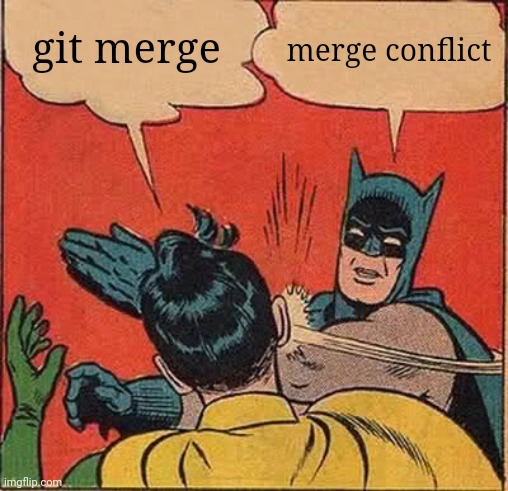
\includegraphics[width=0.7\textwidth,height=0.9\textheight]{figures/mergeConflict.jpg}
  \end{center}
\end{frame}

\begin{frame}[fragile]{How to Resolve Merge Conflicts}
  \begin{block}{What is a Merge Conflict?}
    Happens when Git cannot automatically merge because two branches edit the \textbf{same line} or one deletes a file the other modified.
  \end{block}
    
  \begin{columns}
    \begin{column}{0.5\textwidth}
      \begin{alertblock}{Step-by-Step Resolution}
        \begin{enumerate}
          \item Open the conflicted file(s)
          \item Look for conflict markers:
          \begin{itemize}
            \item \texttt{<<<<<<< HEAD} (your changes)
            \item \texttt{=======}
            \item \texttt{>>>>>>> branch-name} (their changes)
          \end{itemize}
          \item Edit code to keep desired changes \& remove markers
          \item Save the file
          \item Stage the resolved file: \texttt{git add <file>}
          \item Commit the merge: \texttt{git commit}
        \end{enumerate}
      \end{alertblock}
    \end{column}
    \begin{column}{0.45\textwidth}
      \begin{exampleblock}{Example in a File}
\begin{lstlisting}[language=css]
/* style.css */
.title {
<<<<<<< HEAD
  color: blue;
=======
  color: red;
>>>>>>> feature-new-color
}
\end{lstlisting}
      \end{exampleblock}
    \end{column}
  \end{columns}
\end{frame}

\begin{frame}{Key Takeaways}
  \begin{block}{What We've Learned}
    \begin{itemize}
      \item Version control is essential for tracking changes
      \item Git provides a powerful way to manage project history
      \item Basic workflow: modify → stage → commit
    \end{itemize}
  \end{block}

\end{frame}

%--- Session 1 End / Session 2 Begin ---
\begin{frame}
  \centering
  \Huge{\textbf{End of Session 1}}\\[0.5em]
  \large{Next: Session 2 — Collaboration on GitHub}
\end{frame}

\begin{frame}
  \centering
  \Huge{\textbf{Session 2 Begins}}\\[0.5em]
  \large{Collaboration on GitHub}
\end{frame}

% session 2 
%=======================
\section{Session 2: Collaboration on GitHub}
%=======================
\begin{frame}{Session 2: What You'll Learn}
      \begin{block}{GitHub Basics}
        \begin{itemize}
          \item Creating repositories
          \item Pushing code
          \item Basic collaboration
        \end{itemize}
      \end{block}
      
      \begin{center}
        [Space for GitHub screenshot]
      \end{center}
\end{frame}

\begin{frame}{Introduction to GitHub}
  \begin{columns}
    \begin{column}{0.5\textwidth}
      \begin{block}{What is GitHub?}
        \begin{itemize}
          \item A cloud platform for hosting Git repositories
          \item A hub for developer collaboration
          \item The world's largest open-source community
          \item A professional portfolio for your work
        \end{itemize}
      \end{block}
    \end{column}
    \begin{column}{0.48\textwidth}
      \begin{block}{Key Features}
        \begin{itemize}
          \item Code hosting \& version control
          \item Issue tracking
          \item Pull Requests
          \item GitHub Actions (CI/CD)
          \item GitHub Pages
        \end{itemize}
      \end{block}
    \end{column}
  \end{columns}
\end{frame}

\begin{frame}{The Git + GitHub Workflow}
  \begin{block}{Essential Remote Commands}
    \begin{description}
      \item[\texttt{git clone <url>}] Download a repo from GitHub
      \item[\texttt{git push}] Upload committed changes
  \item[\texttt{git pull}] Download \& merge changes
      \item[\texttt{git remote add origin <url>}] Connect local repo to GitHub
    \end{description}
  \end{block}

  \begin{center}
  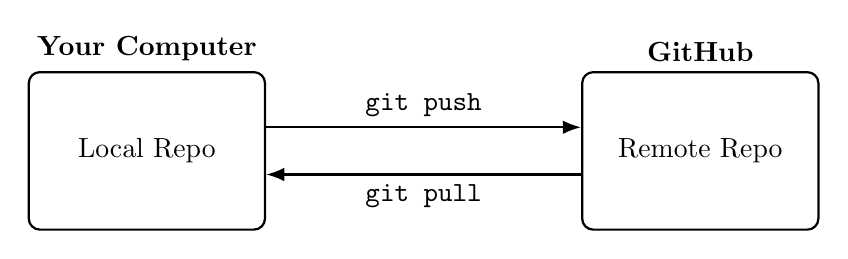
\begin{tikzpicture}[
    node distance=4cm,
    local/.style={rectangle, draw, thick, rounded corners, minimum width=3cm, minimum height=2cm, label=above:\textbf{Your Computer}},
    remote/.style={rectangle, draw, thick, rounded corners, minimum width=3cm, minimum height=2cm, label=above:\textbf{GitHub}},
    arrow/.style={-Latex, thick}
    ]
    \node[local] (local) {Local Repo};
    \node[remote, right=of local] (remote) {Remote Repo};

    \draw[arrow] ($(local.east)+(0,0.3)$) -- node[above] {\texttt{git push}} ($(remote.west)+(0,0.3)$);
    \draw[arrow] ($(remote.west)+(0,-0.3)$) -- node[below] {\texttt{git pull}} ($(local.east)+(0,-0.3)$);
  \end{tikzpicture}
  \end{center}

  \begin{alertblock}{Golden Rule}
    Always \texttt{git pull} before \texttt{git push} to avoid unnecessary conflicts!
  \end{alertblock}
\end{frame}

%--- Session 2 content ---

\begin{frame}{Code Reviews}
  \begin{columns}
    \begin{column}{0.48\textwidth}
      \begin{block}{Reviewing Code: What to Look For}
        \begin{itemize}
          \item Bugs and edge cases
          \item Adherence to code style
          \item Opportunities for improvement
          \item Presence of tests
          \item Clear documentation
        \end{itemize}
      \end{block}
    \end{column}

    \begin{column}{0.48\textwidth}
      \begin{exampleblock}{Giving Good Feedback}
        \begin{itemize}
          \item Be constructive and kind
          \item Explain the 'why' behind suggestions
          \item Ask questions instead of making demands
          \item Offer help if needed
        \end{itemize}
      \end{exampleblock}
    \end{column}
  \end{columns}
\end{frame}

\begin{frame}{Pull Requests (PRs)}
  \begin{block}{What is a Pull Request?}
    A way to propose and discuss changes before merging them into the main project. PRs are the heart of collaboration on GitHub.
  \end{block}

      \begin{block}{The PR Workflow}
        \begin{enumerate}
          \item Push your feature branch to GitHub
          \item Click "New Pull Request" on GitHub
          \item Describe your changes clearly
          \item Request reviews from teammates
          \item Discuss, make more changes if needed
          \item Merge!
        \end{enumerate}
      \end{block}
   
\end{frame}

%--- Session 2 End / Session 3 Begin ---
\begin{frame}
  \centering
  \Huge{\textbf{End of Session 2}}\\[0.5em]
  \large{Next: Session 3 — Common Git Problems}
\end{frame}

\begin{frame}
  \centering
  \Huge{\textbf{Session 3 Begins}}\\[0.5em]
  \large{Common Git Problems}
\end{frame}

%=======================
\section{Session 3: Common Git Problems}
%=======================

\begin{frame}[fragile]{Common Git Problems \& Fixes}
  \begin{block}{"I committed to the wrong branch!"}
    \begin{itemize}
        \item \textbf{Scenario:} Accidentally committed on `main` instead of your feature branch
        \item \textbf{Fix:}
        \begin{enumerate}
            \item Create the correct branch: \verb|git branch feature-branch|
            \item Reset main back one commit: \verb|git reset HEAD~ --hard|
            \item Switch to your branch: \verb|git checkout feature-branch|
            \item Commit is now safely on the correct branch
        \end{enumerate}
    \end{itemize}
  \end{block}

  \begin{alertblock}{"I need to undo my last commit!"}
     \begin{itemize}
         \item Keep changes but undo commit: \verb|git reset HEAD~|
         \item Permanently delete last commit: \verb|git reset HEAD~ --hard| (caution!)
     \end{itemize}
  \end{alertblock}
\end{frame}


%=======================
\section{Conclusion}
%=======================

\begin{frame}{Conclusion \& Next Steps}
    \begin{block}{What You've Learned}
        \begin{itemize}
            \item Git fundamentals \& version control
            \item Using branches for parallel development
            \item Collaborating on GitHub via Pull Requests
            \item Handling merge conflicts \& common issues
        \end{itemize}
    \end{block}

    \begin{exampleblock}{Your Journey Forward}
        \begin{itemize}
            \item Practice Git commands daily
            \item Start a personal project on GitHub
            \item Contribute to open-source projects
        \end{itemize}
    \end{exampleblock}
\end{frame}

\begin{frame}
  \centering
  \Huge{\textbf{Thank You!}}\\[1em]
  \large{Questions or feedback?}
\end{frame}

\end{document}
